\documentclass{book}

\usepackage{graphicx}

\begin{document}

\setcounter{chapter}{-1}

\title{Software Craftsmanship for the Curious Craftsperson}
\author{David Souther}
\maketitle

\pagenumbering{roman}
\tableofcontents
\newpage

\pagenumbering{arabic}

\chapter{Introduction}

Human endeavors rest on the backs of the hard-working crafters. From stone-
movers of the Egyptian pyramids to steel-workers on today's oil rigs, skilled
workers built civilization with their hands. Stone, steel, lumber, and leather
have for centuries been the foundation of human enterprise. In the 21st
century, there is a new medium demanding attention: information. The data
flying across the Internet is the backbone of international trade and
commerce, and needs skilled craftspeople to shape it. Yet even as professional
carpenters build masterwork cabinetry for law firms and movie stars, there are
laymen working on the same craft with the same tools in their garage. This is
no less true for computers --- the relatively low cost of consumer software
gives hobbyist programmers the same tools to work with as the professional.

This book is aimed at those who are interested in this new medium as a
potential hobby or curiosity. The book begins assuming the reader knows how to
turn on and use their computer for basic tasks --- email, word processing,
image editing, and video games, and takes them to a level where they will be
comfortable and confident in using and controlling their computers. This book
is very fast paced. Software development is a field which has undergone active
development for the past 80 years, yet did not exist beyond a dream before
then. There is a lot to learn about this craft, but readers who want to become
truly skilled at this craft will hopefully find this book gives them many of
the tools they need to feel comfortable working their computer. To get the
most out of the text,  I recommended readers work through the companion
workbook. Like any craft, to get good at software development you need to
develop software. The workbooks lead you through developing software, in a way
highlights the concepts presented in the text.

If the book seems hard, fear not. Rome wasn't built in a day, and research
shows it takes ten years of practicing a skill to truly develop expertise.
This book is one way to approach learning this subject, which hopefully will
work for you. If not, one of the many references in the bibliography might
provide a different approach that works better for you.

\section{Computers Are Tools}

Information is a critical piece of today's infrastructure. How people  use
information is part of the field of Computer Science. Computer Science is on
the one hand deeply seated in mathematics, and on the other, firmly rooted in
practicality. The computer itself is simply a tool, like a band saw or plasma
torch, which do amazing things with this data. Whether used in large-scale
data mining and predictions for financial institutions, determining exactly
what websites have what content, or creating a side show of family photos. At
the end of the day, the laptop or desktop sitting in front of you is just a
piece of silicone, copper, and plastic, capable of doing only exactly what it
is told.

The task of the computer programmer is to tell the computer what to do. This
is not an easy task. When people think about a problem, we can start off being
a bit loose on how we describe the problem to ourselves. We can find issues or
errors in our assumptions, and change them on the fly. Computers cannot do
this. Every condition must be considered before hand. Say you're balancing
your check book. You add up \$12.57, \$52.45, and \$1.99, but miss the decimal
on the \$52.45, and end up with \$5249.56 --- clearly an error. On paper, it
is obvious what you did wrong. The computer has no way of knowing this was an
error. Instead, it is up to the good programmer to tell the computer to verify
that any numbers typed into the financial program ends with a decimal and two
numbers. Then, the program can warn the user before making the calculation,
potentially avoiding a costly transaction.

\subsection{How to use this tool}

Software craftsman use this tool by writing programs. A program is a document
both written and read by human beings, while telling the computer
unambiguously what to do. Take this example: $4 + 6 / 2$. Is the answer 7 or
5? If you remembered something like ``Please Remember My Dear Aunt Sally" from
grade school, you would say 7. If you were a desk calculator in an
accountant's office, you would say 5. This statement is {\it ambiguous} --- it
could mean more than one thing. The programmer's job is to decide if the
statement should be $(4 + 6) / 2 = 5$ or $4 + (6 / 2) = 7$.

Of course, this is a minor pedantic exercise. As software gets more complex,
the question becomes ``how does the computer help people interact with their
data?" Facebook is an excellent tool for managing data regarding many aspects
of your relationships with friends and relatives online, by making it very
easy to share photos and other tidbits of information. Microsoft Word is an
excellent program to enable people to write documents, vital pieces of data
for business, education, and private correspondence. Clearly, there is much to
consider when writing a program --- when using the tools of software
craftsmanship.

\subsection{How to share this tool}

There is a whole world outside your front doorstep, and as much as some
programmers might want to deny it, at some point every craftsman's programming
will be used by someone else. It is important your code be both readable and
usable by these other craftsmen. There are many ways to do this, and many
great tools to facilitate this. While many software craftsman may want to
hoard their code, this is simply not possible. Even at companies like
Microsoft, the largest proprietary software development company on the planet,
teams are used because software projects, even most hobbyist projects, are too
large for one person to handle alone.

Many computer science courses ignore this aspect of programming, which I
believe is a real detriment to the students. Many computer science students
can go their entire undergraduate careers without ever looking at their peer's
code, and only having their program reviewed by the instructors. Craftsman of
all fields can drastically improve their work by meeting and sharing ideas.
Building partnerships with other craftsmen is one of the most rewarding ways
to practice a trade, but can also be a harrowing experience learning how to
work and interact with a completely new group of people. To work past this
impediment, I present tools for managing and sharing your programs early in
the book (Chapter 3, Source Control), and encourage you to find other
programmers and technology clubs in your area and on the Internet.


\section{Computer Languages}

Computer languages are the tie between the world of everyday common sense
conversation and the exact stupidity of the computer. There are hundreds, if
not thousands, of different programming languages today. Many are ``toy"
languages, built for a fun exercise or class project and are not intended for
wide-scale use. There are other languages that are proven as the working
horses of computers, and are used everywhere from your cell phone to robots
running on Mars.

Languages are often classed based on their style of programming, and their
level of expressivity. There are, broadly, three styles of programming:
imperative, functional, and logical. Imperative languages are similar to a
cookbook recipe. They describe, one statement at a time, the ``things" a
computer is to do---add two numbers, print those numbers to the screen, ask
the user for confirmation. C, JavaScript, and Python are all imperative
languages. Functional languages embrace the mathematics of computer science.
Functional languages often use similar syntactic constucts as imperative
languages, but with fundamental underlying differences. Haskell is a
functional programming language. Logical programming languages have little to
do with either imperative or functional programming. Prolog is a logical
programming language. Logical programming will not be discussed in this book.

Expressivity is notion for the ratio of amount of programming code written to
how much the computer does. Languages with the least amount of expressivity
are referred to as ``low-level" languages --- they must deal with all aspects
of the computer and its memory. ``High-level" languages handle many of the
details of working on computer hardware, and let the programmer just focus on
expressing the logic of the program in question. This book is presented using
three different languages. These languages were chosen because they each
represent a very different approach to software craftsmanship. Each approach
is correct in  its own way, and it is important to know each of the approaches
to be a great software craftsman. Further, each of these three languages is
mature, and actively used in a variety of projects today.

\subsection{C}

C started its life at Bell Labs in 1973. C was written by Dennis Kernighan and
Brian Ritchie as a language to write the Unix operating system in. Before C,
operating systems (the program enabling all the other programs to run) were
written in an assembly language for each computer Unix would run on. However,
no two brands of computers had the same assembly language, so any time someone
wanted to run Unix on a new computer, they had to rewrite the entire operating
system. At the time, this could be thousands of lines of code. Today, it would
take millions of lines of assembly to code Windows or Linux. C was designed to
be a consistent language that, rather than being run on a computer as is,
would first be compiled into the appropriate assembly code.

C is widely considered the ``lowest-level" of today's common programming
languages, meaning C is as close to running ``on the hardware" as you can get.
When writing C, the programmer has to deal with many aspects of computer
memory management. There are few utilities to achieve all but the most common
tasks (though there are a wealth of ``libraries" to fill the gap). C is the
only language used in this book that must be compiled before being run. This
``low-level" nature of C makes it a very powerful language, especially when
faced with requirements to interact directly with hardware, or when hardware
is in short supply (embedded on robots or cell phones). That power comes with
great responsibility for writing the program correctly.

\subsection{Python}

Python is a programming language developed by Guido van Rossum in the late
1980s. Python has gone through two major revisions since its first release,
and now is widely available on nearly any computing platform. Today, Python is
used by many Linux distributions to write a variety of their higher-level
tools. Organizations from Google to NASA use Python for a variety of their
mission-critical applications.

Python was designed to be a very flexible language, and as such is high-level
compared to C. Python was also designed to be a fun language to use---the name
Python refers not to the snake, but to Monty Python's Flying Circus. Python
has a certain culture around its use not seen in many other programming
languages. In Python, the prevailing wisdom is ``there should be one---and
preferable only one---obvious way to do it."

\subsection{Javascript}

Javascript is a programming language developed at Netscape in 1994 by Brandon
Eiche over the course of a week. Javascript is the de-facto standard for
writing programs served over the Internet to run in a user's web browser.
While actually a functional programming language, Javascript is often
(mis)represented as being an imperative language. This has lead to some very
poor code being written in the 15 plus years since its inception. That said,
its use in every web browser today has many people working to make Javascript
a less-maligned and better respected language.

Javascript is a very high level language. The programmer has few worries about
memory management, and no capabilities to access the computer's hardware
(though there are initiatives to enable such use). When combined with
libraries like jQuery, javascript can be the most expressive of the three
languages presented. When we start working with graphical programs later in
the book, Javascript's expressive power will really shine, in that the amount
of code needed to do the same thing (click a button) can often be an order of
magnitude less than a similar program in C.

\section{Overview of the Text}

\subsection{Syntactic Core (1--4)}

The first four chapters will cover the core of writing programs. This will get
readers to the point where they can have their computer talking to them and
asking questions, though perhaps not gracefully. This section also covers the
basics of source control, and sharing code between developers.

\subsection{Programming Patterns (5--9)}

The second section covers patterns in software craftsmanship---commonly used
ideas which can be the large building blocks of a program's design. This
includes discussions on modeling data, saving data, and some ideas on how to
make good program design decisions. This section also includes a chapter on
debugging---finding out what went wrong with a program (things will go wrong).

\subsection{Building Large Programs (10--13)}

The last section deals with managing large pieces of software. The section
will go through building a basic ``paint" application, where users can draw
lines and colors on a canvas, and save the painting to look at later. This
section also includes a chapter on how to work with other people on the same
project.

\subsection{Appendices: Tools for the Toolmakers}

Any craftsman needs a workbench that suits their needs. The appendices address
several aspects around such a workbench. First and foremost, programs are
text. As such, it is important to use a text editor that facilitates looking
at and `seeing' your code. Second is a discussion of the Linux operating
system. Its open source nature encourages users to take responsibility for
their computer, and provides a wealth of tools for programming unavailable (or
at least difficult (read, costly) to acquire) on Windows. Finally, there is a
discussion on computer hardware. This is a look at what physically is going on
in your program, focusing on the CPU, memory, and some peripherals. This is
not strictly critical for learning software programming as a craft, but
hopefully you will be interested enough by the end of the book to want to take
a deeper look at what's going on.

\section{Workbooks}

Like any skill, software craftsmanship takes practice. The workbooks are
designed to highlight the concepts presented in the text, while giving you an
opportunity to practice these skills. The workbooks are broken into lessons
roughly corresponding to sections of the main text. Each lesson has two parts.
The first part is a listing of code. You should type the code into your editor
exactly as written. Do not copy and paste the code. Much of programming
involves paying very close attention to a myriad of small details, and every
character has meaning. This discipline in typing code exactly as presented
will pay off in your programming future. The second part of each lesson is a
few exerices to work with the new concepts in the lesson, and combine them
with what you learned and wrote previously. Some of the lesson exercises will
involve conducting research on the internet. Being able to find help with
programming questions is another invaluable skill as a software developer.


\part{Syntactic Core}
\chapter{Basic Types and Control Flow}

Computers work with data. At the lowest level, this data is just `on' and
`off' in a transistor. Software craftsmen don't work at this level. Instead,
our programming languages give us the tools to work with this data in a much
more intuitive fashion. In broad strokes, this is achieved with two concepts:
data types and control flow. Data types describe the data our program is
working with, whether it be a number, a bank account, or an image. Control
flow describes the operations that occur on the data over time, like adding
numbers, checking the balance of a bank account, or cropping an image.

You can think of data types as the space of a program. At any one point in
time, we will have certain sets of data we are working with. We can stop the
program, look at the data, and carry on. While we think of three dimensions in
space,  up/down, left/right, and front/back, there are many more dimensions we
could talk about for different things. A table has a color, along with its
position. Our programs represent these properties in different ways, but we as
programmers abstract them, and the term we use to talk about these properties
is data types.

Control flow would then be the time aspect of a program. As the program runs,
it does different things to the data. At some point, it might need to make a
decision, and do one thing or another depending on what properties the data
has. At another point, the program might need to do the same thing on a bunch
of similar pieces of data. Control flow represents the logical actions our
programs follow.

\section{Syntax}

Before we dive into discussing our first program, there is one more topic to
cover. Syntax describes the words and symbols that make a valid program. In
English, nouns, verbs and adjectives must come in a certain fashion for a
sentence to make sense. In a computer program, there are similar rules for how
a program can be written, and still make sense to the computer to run. We will
cover the details of syntax for each programing language in the workbook, but
there are some key terms to know regardless of the language.

\subsection{Keywords}

In any programming language, there are a few reserved {\it keywords} --- words
which have a specific meaning to the program. Most programming languages only
use no more than a couple dozen keywords. These will be covered in the
workbooks as needed.

\subsection{Variables}

In a program file, variables are words used to refer to some piece of data.
Variables let programmers use concrete concepts to refer to the more abstract
realm of the mathematical values in the computer. Variables can generally be
any word that isn't a keyword in a programming language.

\subsection{Operators}

Operators are the built-in things that can happen to data. Common operators
are things from elementary arithmetic --- add {\tt +}, subtract {\tt -},
multiply {\tt *}, and divide {\tt /}. Other operators let the program compare
two pieces of data --- equals ({\tt ==}), less-than ({\tt <}), greater-than-
or- equal-to ({\tt >=}). Notice there are some funny things for the comparison
operators. First, equals is two characters, {\tt ==}, not the single {\tt =}
used in elementary school. This is because a single {\tt =} sign is an
operator used to assign values to a variable. Multiplication is a star, {\tt
*}. While {\tt x} was used in elementary school, we use {\tt *} for our
programs because {\tt x} could be a variable, and we need to be unambiguous in
what the program means. There is no $\le$ on a common keyboard, so programs
use the two character combinations of {\tt <=} and {\tt >=} to do comparisons.
There are other operators that will be covered as they are needed.

\section{Basic Types}

Data Types fall into two distinct categories. `Primitive' data types are those
that are specified in the programming language itself. `Complex' data types
are defined by the programmer, and are made up entirely of primitive data
types and other complex data types already defined. In this section, we will
go over the basic data types in your language. In general, these basic types
are applicable in any programming language in major use today, with small
discrepencies between them.

\subsection{Numbers}

Since computers only do arithmetic, everything is at some level a number in
the computer. In mathematics, numbers can be as big as they need to be. If we
were counting pebbles of sand on a beach, there is a number to represent that
(though I will not be the one doing the counting). Computers are somewhat more
finite. The representation of a basic number in a computer is confined to a
range of a few possible values. On today's computers, that range is either
$2^32$ or $2^64$ possible values. The 32 and 64 refer to the number of `bits'
your computer handles. When the IT guy asks whether your computer is 32 or 64
bit, this is what we're talking about.

\subsubsection{Integers}

Integers in computer programming are Whole Numbers from elementary school ---
1, 5, -15, 47. They can be positive or negative. In some languages, they are
limited in size based on your computer's processor. On a 32 bit computer, the
range of integers is from $-2^{31}$ (-2 147 483 648) to $2^{31}-1$ (2 147 483
647) (the one positive number is lost for 0). On a 64 bit computer, the range
of values is $-2^{63}$ to $2^{63}-1$. It is left to the reader to determine
those numbers in base 10. Integers are useful in many cases because they are
very easy to work with, but have a major drawback of being unable to work with
fractional parts. That is the use of Floating-point numbers.

\subsubsection{Floats}

In your computer, there is only so much room to store numbers. As mentioned in
the previous section on integers, there are only $2^32$ possible numbers you
can represent on a 32-bit computer. Those integers are only whole numbers, and
can't represent a number like $\frac{1}{2}$ or $\pi = 3.1415926...$. Instead,
we use a special type of number called a {\em Floating Point} number. A
floating point number can still only represent $2^32$ different values, but it
is interpreted in such a way that it can represent fractional numbers. At this
point, we must take a detour into the world of mathematics in order to
understand how floating point numbers work, and in the process save ourselves
from making some very costly mistakes.

{\bf Floating Point Arithmetic}\
This section explains some complicated math.\

Our everyday number system is a base-10 number system. When you write your
numbers, you write 1, 2, 3, 4, 5, 6, 7, 8, 9, 10, 11, 12 $...$. Notice how
starting at 10 we use two characters to represent the number- 1 and 0. ``Well,
duh" you might say. In fact, there is a very specific reason we need two
numbers at this point. What 10 means is $(1 * 10^1) + (0 * 10^0)$. This is the
base-10 system- each character in the numer means $a * 10 ^ p$ where $a$ is
the number, and $p$ is its position (starting from 0). So, the number 347 is
$(3 * 10 ^ 2) + (4 * 10 ^ 1) + (7 * 10^0)$. In a computer, we use binary, or a
base-2 number  system. Instead of writing numbers as $a * 10^p$, we write them
as $a * 2 ^ p$. So, to get 12, we need to write 1100, or $(1 * 2 ^ 3) + (1 *
2^2) + (0*2^1) + (0 * 2 ^ 0) = (1 * 8) + (1 * 4) + (0 * 2) + (0 * 1) = 8 + 4 +
0 + 0 = 12_10$.

We can talk about decimal numbers like 1.56 in the same way--- $(1 * 10 ^ 0) +
(5 * 10 ^ -1) * (6 * 10 ^ -2) = 1 + \frac{5}{10} + \frac{6}{100} =
\frac{100}{100} + \frac{50}{100} + \frac{6}{100} = \frac{156}{100} =
\frac{39}{25}$.

While this math might be disheartening, it is important to remember that
computers do work in this fashion under the hood. That said, this is the only
time this will be discussed in the main book (though some advanced exercises
in the workbook will deal with computer arithmetic in more depth, and appendix
3 is devoted to a discussion of just how the computer does work under the
hood).

\subsection{Characters}

Characters are single bytes of data that are interpreted as being human-
readable in some form. For instance, the letter `a' is the integer 97. The
letter `V' is 86. `!', the exclamation point, is 33. Because the computer
operates on numbers, there is no distinction to it between the number 33 and
the character `!'. Instead, programmers tell their programs how they intend to
use the data, and the program does the ``right thing". The ``right thing" is
exactly what is was told to do. To understand what you're telling the computer
to do better, it is important to know that there is nothing special about the
mappings between the numbers and characters. Indeed, the first 128 character
numbers were chosen by an organization called the American Standard Code for
Information Interchange, or ASCII. For this reason, the first 128 characters
are called the ``ASCII'' character set. Of course, there is no way to fit all
the characters of both the Latin and Cyrillic alphebets into 128 different
numbers, much less most Asian character sets. For this reason, there is
another character set called UNICODE that defines over 4 million possible
characters, enough to satisfy human languages for some time. We will not go
into the details of Unicode here.

%TODO Picture of ASCII 0 - 127
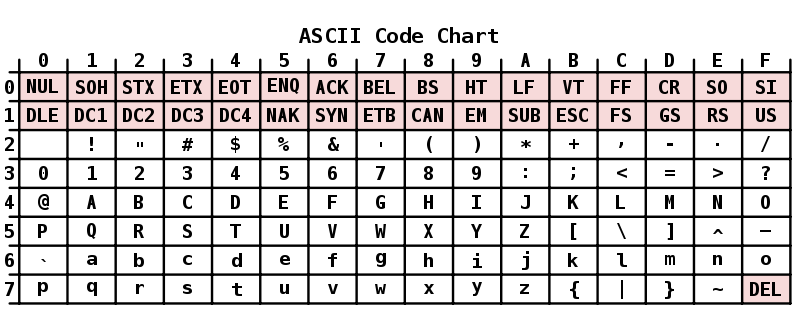
\includegraphics[width=120mm]{./01_basic_types_and_control_flow/800px-ASCII_Code_Chart.png}

Let's take a closer look at some features of the ASCII character set. First,
notice that uppercase and lowercase characters are represented distinctly.
This is why case sensitivity is important on computers. Second, 0 through 31
look really funky. That's because these are called control characters, not
printing characters. Most of these control characters are no longer used in
today's computers (they were used to literally control printers and other
devices in the 70s and 80s), but there are some that warrant special
attention. The first is NULL, 0. NULL is used in C to represent the end of an
array (see Chapter 2). 10, `$\backslash$n' or Newline, is used to make the
computer put a line break in a program's output; otherwise, everything would
show up on one long horizontal line. Second is 15, `$\backslash$r' or Carriage
Return. This goes back to when computer printers were fancy typewriters, which
required a special symbol to move the carriage back to the starting position.
While I can't think of any printers today that need this fuctionality, it is
not uncommon to see `$\backslash$r$\backslash$n' as a legacy pair of
characters in many programs. The last control character that is interesting to
us is 9, `$\backslash$t', horizontal tab. The horizontal tab tells the
computer that we want a lot of whitespace (usually 4 or 8 spaces worth).

\subsection{Strings}

Characters on their own aren't particularly interesting. What is useful is
having long runs of characters to make up words, sentences, paragraphs, and so
on. We achieve this by using what are called strings--- which are literally
just a collection of characters in a row. Usually strings are surrounded by
double quotes in a program. See the workbook for a variety of examples on how
strings look and work in a program.

While characters really are treated as just numbers, strings have a variety of
common operations that don't make sense with numbers. Among these are
operations to determine the length of a string (how many characters it has),
to combine strings together, and to pull strings apart. These are also covered
in detail in the workbook.

\section{Control Flow}

\subsection{Blocks}

\subsubsection{Expression}

\subsubsection{Statement}

\subsection{Branching}

\subsubsection{If-Then-Else}

%\subsubsection{Cases}

\subsection{Looping}

\subsubsection{For Range}

\subsubsection{While}

\section{Comments}

There is one last piece of a program we need to mention. Comments are text in
our programs that are not used by the computer, but are purely for

\chapter{Functions, Arrays, and Strings}

\section{Functions}

\subsection{Procedure}

\subsection{Function}

\subsection{Recursion}

\section{Arrays}

\section{Strings}

\chapter{Source Control}

\section{Tracking}

\section{Sharing}

\section{Fixing Goofs}

\chapter{Introduction to Objects}

\section{Structured Data}

\section{Methods}



\part{Programming Patterns}
\chapter{Object Composition}

\section{Inheritence}

\section{Polymorphism}

\section{Visibility}

\chapter{Debugging}

\section{Logging}

\section{Exceptions}

\section{Breakpoints}

\subsection{Watches}

\chapter{Input \& Output}

\section{Input}

\section{Output}

\section{Parameters}

\section{Command Line}

\section{Files}

\section{Databases}

\chapter{Patterns I: Lazy Loading, Singleton, Iterators}

\section{Lazy Loading}

\section{Singleton}

\section{Iterators}

\chapter{Patterns II: Factory, Decorator, Visitor}

\section{Factory}

\section{Decorator}

\section{Visitor}


\part{Building Large Programs}
\chapter{Unit Testing}

\chapter{Model-View-Controller}

\chapter{MVC Redux}

\chapter{Team Programming}


\part{Appendicies: Tools for the Toolmakes}
\appendix
\chapter{Text Editors}

\section{Vi}

\section{gedit}

\chapter{Linux}

\section{Linux Desktop}

\section{Command Line}

\subsection{Vi}

\subsection{Bash}

\chapter{Computer Hardware}

\section{Computer Arithmetic}

\section{Von-Neuman Machine}

\section{High-Level Assembly}

\section{Memory Hierarchy}


\end{document}

